\subsectionFrame{Introduction to Mobile Communication}

\begin{frame}{What Makes Mobile Communication Hard?}
  \begin{columns}[T,onlytextwidth]
    \begin{column}{0.58\textwidth}
      Requirements
      \begin{itemize}
        \item Reach a user anywhere, without knowing where they are
        \item Keep a call alive while the user moves
        \item Serve many users at the same time
        \item Small, battery-powered terminals at low cost
      \end{itemize}
      \vspace{0.4em}
      Constraints
      \begin{itemize}
        \item Radio spectrum is a finite resource (see Preliminaries)
        \item All users in an area share the same medium
        \item Terminals must work with the networks they encounter
      \end{itemize}
    \end{column}
    \begin{column}{0.38\textwidth}
      \begin{block}{Central Question}
        Why did early mobile communication develop towards \textbf{cellular} and \textbf{digital} systems?
      \end{block}
      \begin{alertblock}{Pattern of this Chapter}
        Each generation removes the bottleneck of the previous one.
      \end{alertblock}
    \end{column}
  \end{columns}
\end{frame}

\begin{frame}{Generations at a Glance}
  \centering
  \begin{tabular}{llll}
    \toprule
    \textbf{Generation} & \textbf{Era} & \textbf{Signal} & \textbf{Characteristic Technology} \\
    \midrule
    \alert{0G} & \alert{from 1946} & \alert{Analog} & \alert{Single high site, few channels} \\
    \alert{1G} & \alert{from 1979} & \alert{Analog} & \alert{Cellular reuse, \acrshort{acro:fdma}} \\
    \alert{2G} & \alert{from 1991} & \alert{Digital} & \alert{\acrshort{acro:tdma} (\acrshort{acro:gsm})} \\
    3G & around 2000 & Digital & \acrshort{acro:cdma} \\
    4G & around 2010 & Digital & \acrshort{acro:ofdm} (\acrshort{acro:lte}) \\
    5G & around 2020 & Digital & \acrshort{acro:ofdm} (\acrshort{acro:nr}) \\
    6G & around 2030 (expected) & Digital & In standardization \\
    \bottomrule
  \end{tabular}

  \vspace{1em}
  This lecture covers the highlighted generations.
\end{frame}


\subsectionFrame{0G and the Capacity Problem}

\begin{frame}{0G: Mobile Radio Telephony}
  \begin{columns}[T,onlytextwidth]
    \begin{column}{0.54\textwidth}
      United States~\cite{young-amps}
      \begin{itemize}
        \item 1946: Public mobile telephone service in St.\ Louis
          \begin{itemize}
            \item Three channels near \qty{150}{\mega\hertz}
            \item Calls handled by a mobile operator
          \end{itemize}
        \item 1964: \gls{acro:imts}
          \begin{itemize}
            \item Automatic channel selection
            \item Customers dial themselves
          \end{itemize}
      \end{itemize}
      \vspace{0.4em}
      Common Properties
      \begin{itemize}
        \item Analog transmission
        \item Vehicle-mounted terminals
        \item One high site covers a whole city or region
      \end{itemize}
    \end{column}
    \begin{column}{0.42\textwidth}
      \begin{block}{Germany}
        \begin{itemize}
          \item \textbf{A-Netz} (1958): manually switched, peak of about \num{10800} subscribers~\cite{a-netz}
          \item \textbf{B-Netz} (1972): direct dialing, peak of about \num{27000} subscribers in 1986~\cite{b-netz}
        \end{itemize}
      \end{block}
    \end{column}
  \end{columns}
\end{frame}

\begin{frame}{0G: The Capacity Bottleneck}
  \begin{columns}[T,onlytextwidth]
    \begin{column}{0.5\textwidth}
      \begin{itemize}
        \item One site occupies a channel in its entire coverage area
        \item Capacity = number of channels, regardless of area
        \item Only a few dozen channels available in many areas~\cite{young-amps}
        \item Demand exceeds supply: prospective customers end up on backlog lists~\cite{young-amps}
      \end{itemize}
      \alert{Remark:} Better equipment helps only slightly. Halving the channel spacing at \qty{150}{\mega\hertz} raised 6 channels to 11~\cite{young-amps}.
    \end{column}
    \begin{column}{0.46\textwidth}
      \centering
      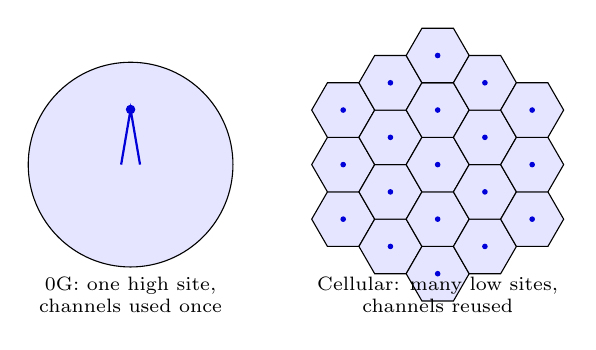
\begin{tikzpicture}[>=latex]
    \def\hexcell#1#2{\draw[fill=blue!10, shift={(#1,#2)}] (0:0.4) -- (60:0.4) -- (120:0.4) -- (180:0.4) -- (240:0.4) -- (300:0.4) -- cycle;}

    % 0G: one tower covers the whole area
    \draw[fill=blue!10] (0,0) circle (1.3);
    \draw[thick, blue!85!black] (-0.12,0) -- (0,0.7) -- (0.12,0);
    \filldraw[blue!85!black] (0,0.7) circle (1.5pt);
    \node[font=\scriptsize, align=center] at (0,-1.65) {0G: one high site,\\channels used once};

    % Cellular: many low sites
    \foreach \q in {-2,...,2} {
        \foreach \v in {-2,...,2} {
            \pgfmathtruncatemacro{\dist}{max(abs(\q),abs(\v),abs(\q+\v))}
            \ifnum\dist<3
                \pgfmathsetmacro{\cx}{3.9+0.6*\q}
                \pgfmathsetmacro{\cy}{0.6928*(\v+0.5*\q)}
                \hexcell{\cx}{\cy}
                \filldraw[blue!85!black] (\cx,\cy) circle (0.8pt);
            \fi
        }
    }
    \node[font=\scriptsize, align=center] at (3.9,-1.65) {Cellular: many low sites,\\channels reused};
\end{tikzpicture}

      \begin{block}{Key Idea}
        Lower the transmit power and the same channel can be reused nearby.
      \end{block}
    \end{column}
  \end{columns}
\end{frame}


\subsectionFrame{The Cellular Concept}

\begin{frame}{Cellular Concept I}
  \begin{columns}[T,onlytextwidth]
    \begin{column}{0.58\textwidth}
      Frequency Reuse
      \begin{itemize}
        \item Divide the service area into small cells
        \item Each cell uses a subset of the available channels
        \item A cluster of $N$ cells uses all channels once
        \item Distant cells reuse the same channels
        \item Concept formulated by D.\,H.\ Ring in 1947~\cite{young-amps}, first deployed decades later
      \end{itemize}
      \vspace{0.4em}
      Handover and Cell Splitting
      \begin{itemize}
        \item Handover: ongoing call moves to the next cell
        \item Cell splitting: smaller cells where demand grows, capacity scales with demand~\cite{macdonald-cellular}
      \end{itemize}
    \end{column}
    \begin{column}{0.38\textwidth}
      \begin{figure}
        \centering
        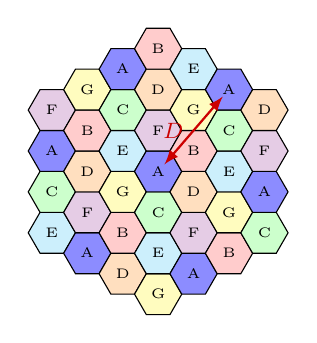
\begin{tikzpicture}[>=latex]
    \colorlet{cell0}{blue!45}
    \colorlet{cell1}{red!20}
    \colorlet{cell2}{green!20}
    \colorlet{cell3}{orange!25}
    \colorlet{cell4}{cyan!20}
    \colorlet{cell5}{violet!20}
    \colorlet{cell6}{yellow!25}
    \def\hexcell#1#2#3{\draw[fill=#3, shift={(#1,#2)}] (0:0.3) -- (60:0.3) -- (120:0.3) -- (180:0.3) -- (240:0.3) -- (300:0.3) -- cycle;}

    % Hexagonal grid, cells with the same letter share one channel set (N = 7)
    \foreach \q in {-3,...,3} {
        \foreach \v in {-3,...,3} {
            \pgfmathtruncatemacro{\dist}{max(abs(\q),abs(\v),abs(\q+\v))}
            \ifnum\dist<4
                \pgfmathtruncatemacro{\c}{mod(mod(\q+5*\v,7)+7,7)}
                \pgfmathsetmacro{\cx}{0.45*\q}
                \pgfmathsetmacro{\cy}{0.5196*(\v+0.5*\q)}
                \hexcell{\cx}{\cy}{cell\c}
                \node[font=\tiny] at (\cx,\cy) {\ifcase\c A\or B\or C\or D\or E\or F\or G\fi};
            \fi
        }
    }

    % Co-channel distance between two "A" cells: axial offset (2,1)
    \draw[<->, thick, red!80!black] (0.08,0.09) -- (0.82,0.95)
        node[midway, left, font=\footnotesize, text=red!80!black] {$D$};
\end{tikzpicture}

        \caption{Reuse pattern for $N=7$}
      \end{figure}
      \begin{block}{Channels per Cell}
        \centering
        $S_\mathrm{cell} = S_\mathrm{total} / N$
      \end{block}
    \end{column}
  \end{columns}
\end{frame}

\begin{frame}{Cellular Concept II}
  \begin{columns}[T,onlytextwidth]
    \begin{column}{0.54\textwidth}
      Reuse Geometry
      \begin{itemize}
        \item Hexagonal grid allows $N = i^2 + ij + j^2$ with $i,j \in \mathbb{N}_0$
        \item Co-channel reuse ratio $D/R = \sqrt{3N}$
      \end{itemize}
      \vspace{0.4em}
      Co-Channel Interference
      \begin{itemize}
        \item Received power decays as $P \propto d^{-n}$ with path loss exponent $n$
        \item First tier: six interferers at distance $\approx D$
        \item User at the cell edge, distance $R$ to serving site
        \item Independent of $R$ and of the transmit power
      \end{itemize}
      \alert{Tradeoff:} Small $N$ gives more channels per cell but less \gls{acro:sir}.
    \end{column}
    \begin{column}{0.42\textwidth}
      \begin{block}{Downlink \gls{acro:sir} Estimate}
        \centering
        $\dfrac{S}{I} \approx \dfrac{R^{-n}}{6 D^{-n}} = \dfrac{\left(\sqrt{3N}\right)^n}{6}$
      \end{block}
      \begin{block}{Example for $n = 4$}
        \centering
        \begin{tabular}{rrr}
          \toprule
          $N$ & $D/R$ & $S/I$ in dB \\
          \midrule
          3 & 3.0 & 11.3 \\
          4 & 3.5 & 13.8 \\
          7 & 4.6 & 18.7 \\
          12 & 6.0 & 23.3 \\
          \bottomrule
        \end{tabular}
      \end{block}
    \end{column}
  \end{columns}
\end{frame}

\begin{frame}{Cellular Concept III}
  \centering
  Live demo: \gls{acro:sir} and capacity versus cluster size
  \begin{itemize}
    \item scripts/section-2/cellular-sir.py
  \end{itemize}
\end{frame}


\subsectionFrame{1G: Analog Cellular Systems}

\begin{frame}{Frequency Division Multiple Access}
  \begin{columns}[T,onlytextwidth]
    \begin{column}{0.54\textwidth}
      \Gls{acro:fdma}
      \begin{itemize}
        \item Each active user gets a dedicated frequency channel
        \item Continuous transmission for the whole call
        \item Simple receivers: filter out one channel
        \item Natural fit for analog \gls{acro:fm} voice
      \end{itemize}
      \vspace{0.4em}
      Consequences
      \begin{itemize}
        \item Channel width sets the capacity directly
        \item Guard bands and sharp filters required
        \item Base station needs one transceiver per channel
      \end{itemize}
    \end{column}
    \begin{column}{0.42\textwidth}
      \begin{figure}
        \centering
        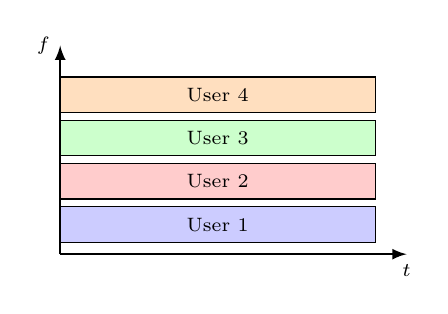
\begin{tikzpicture}[>=latex]
    \foreach \u/\col in {0/blue!20, 1/red!20, 2/green!20, 3/orange!25} {
        \draw[fill=\col] (0,{0.15+0.55*\u}) rectangle (4,{0.6+0.55*\u});
        \pgfmathtruncatemacro{\usernum}{\u+1}
        \node[font=\scriptsize] at (2,{0.375+0.55*\u}) {User \usernum};
    }
    \draw[->, thick] (0,0) -- (4.4,0) node[below, font=\scriptsize] {$t$};
    \draw[->, thick] (0,0) -- (0,2.65) node[left, font=\scriptsize] {$f$};
\end{tikzpicture}

        \caption{Time-frequency resources in \gls{acro:fdma}}
      \end{figure}
      \begin{block}{Example: AMPS}
        \centering
        \qty{30}{\kilo\hertz} channels\\
        Reuse with $N = 7$~\cite{macdonald-cellular}
      \end{block}
    \end{column}
  \end{columns}
\end{frame}

\begin{frame}{1G Systems}
  \begin{columns}[T,onlytextwidth]
    \begin{column}{0.56\textwidth}
      \centering
      \begin{tabular}{lll}
        \toprule
        \textbf{System} & \textbf{Region} & \textbf{Start} \\
        \midrule
        NTT & Japan & 1979 \\
        \acrshort{acro:nmt} & Nordic countries & 1981 \\
        \acrshort{acro:amps} & USA & 1983 \\
        \acrshort{acro:tacs} & United Kingdom & 1985 \\
        C-Netz & Germany & 1985 \\
        Radiocom 2000 & France & 1985 \\
        \bottomrule
      \end{tabular}
    \end{column}
    \begin{column}{0.40\textwidth}
      \begin{alertblock}{Fragmentation in Europe}
        \begin{itemize}
          \item National systems, mutually incompatible
          \item Terminals stop working at the border
          \item Small markets keep terminal prices high
        \end{itemize}
      \end{alertblock}
    \end{column}
  \end{columns}
  \vspace{1em}
  \begin{itemize}
    \item Exception: \gls{acro:nmt} was developed jointly and allowed roaming across the Nordic countries
    \item Germany: C-Netz grew to about \num{850000} subscribers~\cite{c-netz}, far beyond A- and B-Netz
    \item Cellular solved capacity, but no system solved compatibility
  \end{itemize}
\end{frame}

\begin{frame}{Limits of 1G}
  \begin{columns}[T,onlytextwidth]
    \begin{column}{0.58\textwidth}
      \begin{itemize}
        \item Analog voice degrades directly with interference
          \begin{itemize}
            \item AMPS targets \qty{18}{\decibel} over \qty{90}{\percent} of the area~\cite{macdonald-cellular}
            \item Requirement forces a large cluster size
          \end{itemize}
        \item No confidentiality
          \begin{itemize}
            \item Calls can be overheard with a scanner receiver
          \end{itemize}
        \item Voice only
          \begin{itemize}
            \item No native data or messaging service
          \end{itemize}
        \item Limited options for further capacity
          \begin{itemize}
            \item One transceiver per call
            \item Speech cannot be compressed in analog form
          \end{itemize}
      \end{itemize}
    \end{column}
    \begin{column}{0.38\textwidth}
      \begin{block}{Next Bottleneck}
        \centering
        Cellular gives capacity by reuse, but the required \gls{acro:sir} limits how tight the reuse can be.
      \end{block}
    \end{column}
  \end{columns}
\end{frame}


\subsectionFrame{2G: Digital Cellular Systems}

\begin{frame}{Analog vs.\ Digital I}
  \centering
  \begin{tabular}{lll}
    \toprule
    & \textbf{Analog (1G)} & \textbf{Digital (2G)} \\
    \midrule
    Voice & Frequency-modulated waveform & Compressed bit stream \\
    Interference & Directly audible & Corrected up to a threshold \\
    Tolerated \gls{acro:sir} & about \qty{18}{\decibel} & about \qty{9}{\decibel} \\
    Confidentiality & None & Encryption \\
    Services & Voice & Voice, messaging, data \\
    Base station & One transceiver per call & Several calls per transceiver \\
    Terminals & Analog circuits & Digital signal processing \\
    \bottomrule
  \end{tabular}

  \vspace{1em}
  \raggedright
  See also \enquote{Why do we have Digital Communication Systems?} in the Preliminaries.

  \alert{Remark:} Digital processing became affordable only with progress in integrated circuits.
\end{frame}

\begin{frame}{Analog vs.\ Digital II}
  \begin{columns}[T,onlytextwidth]
    \begin{column}{0.58\textwidth}
      Capacity in about \qty{25}{\mega\hertz} per direction
      \begin{center}
        \begin{tabular}{lrr}
          \toprule
          & \textbf{AMPS} & \textbf{GSM} \\
          \midrule
          Carrier spacing & \qty{30}{\kilo\hertz} & \qty{200}{\kilo\hertz} \\
          Voice channels per carrier & 1 & 8 \\
          Spectrum per channel & \qty{30}{\kilo\hertz} & \qty{25}{\kilo\hertz} \\
          Total channels & 832 & 992 \\
          Required \gls{acro:sir} & \qty{18}{\decibel} & \qty{9}{\decibel} \\
          Cluster size $N$ & 7 & 4 \\
          \midrule
          \textbf{Channels per cell} & \textbf{119} & \textbf{248} \\
          \bottomrule
        \end{tabular}
      \end{center}
      \footnotesize Simplified: full-rate speech, no sectorization, control channels ignored. AMPS channels were split between two operators.
    \end{column}
    \begin{column}{0.38\textwidth}
      \begin{alertblock}{Main Result}
        Digital roughly doubles capacity, although the spectrum per voice channel barely changes.
      \end{alertblock}
      \begin{block}{Reason}
        Lower required \gls{acro:sir} permits tighter reuse: $N=7 \rightarrow N=4$
      \end{block}
    \end{column}
  \end{columns}
\end{frame}

\begin{frame}{Time Division Multiple Access}
  \begin{columns}[T,onlytextwidth]
    \begin{column}{0.54\textwidth}
      \Gls{acro:tdma}
      \begin{itemize}
        \item Several users share one carrier in turns
        \item User transmits short bursts in an assigned time slot
        \item Requires digital signals: speech is buffered between bursts
        \item Requires time synchronization between users
      \end{itemize}
      \vspace{0.4em}
      Advantages over Pure \gls{acro:fdma}
      \begin{itemize}
        \item One transceiver serves several calls
        \item Terminal does not transmit and receive simultaneously
        \item Idle slots allow measuring neighbor cells before handover
      \end{itemize}
    \end{column}
    \begin{column}{0.42\textwidth}
      \begin{figure}
        \centering
        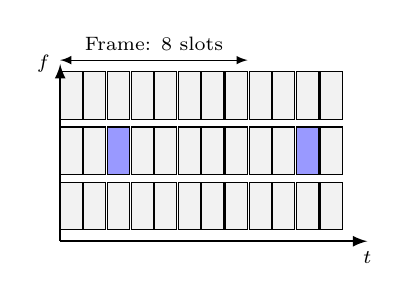
\begin{tikzpicture}[>=latex]
    % Carriers (FDMA) divided into repeating time slots (TDMA)
    \foreach \carrier in {0,1,2} {
        \foreach \slot in {0,...,11} {
            \draw[fill=gray!10] ({0.3*\slot},{0.15+0.7*\carrier}) rectangle ({0.28+0.3*\slot},{0.75+0.7*\carrier});
        }
    }
    % One user occupies the same slot in every frame
    \foreach \slot in {2,10} {
        \draw[fill=blue!40] ({0.3*\slot},0.85) rectangle ({0.28+0.3*\slot},1.45);
    }
    \draw[<->] (0,2.3) -- (2.38,2.3) node[midway, above, font=\scriptsize] {Frame: 8 slots};
    \draw[->, thick] (0,0) -- (3.9,0) node[below, font=\scriptsize] {$t$};
    \draw[->, thick] (0,0) -- (0,2.25) node[left, font=\scriptsize] {$f$};
\end{tikzpicture}

        \caption{Combined \gls{acro:fdma}/\gls{acro:tdma} as used in \gls{acro:gsm}}
      \end{figure}
      \alert{Remark:} \gls{acro:gsm} is a hybrid: carriers separate in frequency, slots separate in time.
    \end{column}
  \end{columns}
\end{frame}

\begin{frame}{GSM Air Interface}
  \begin{columns}[T,onlytextwidth]
    \begin{column}{0.54\textwidth}
      \centering
      \begin{tabular}{ll}
        \toprule
        \textbf{Parameter} & \textbf{Value (GSM 900)} \\
        \midrule
        Uplink band & \qtyrange{890}{915}{\mega\hertz} \\
        Downlink band & \qtyrange{935}{960}{\mega\hertz} \\
        Duplex & \acrshort{acro:fdd}, \qty{45}{\mega\hertz} spacing \\
        Carrier spacing & \qty{200}{\kilo\hertz} \\
        Carriers & 124 \\
        Slots per carrier & 8 \\
        Modulation & \acrshort{acro:gmsk} \\
        Gross bit rate & \qty{270.833}{\kilo\bit\per\second} \\
        \bottomrule
      \end{tabular}
    \end{column}
    \begin{column}{0.42\textwidth}
      \begin{block}{Bit Rate per User}
        \begin{itemize}
          \item Carrier: \qty{270.833}{\kilo\bit\per\second}
          \item Slot share: $\approx\qty{33.9}{\kilo\bit\per\second}$
          \item After burst overhead and control: \qty{22.8}{\kilo\bit\per\second}~\cite{lntwww-gsm}
          \item Protects \qty{13}{\kilo\bit\per\second} speech with channel coding
        \end{itemize}
      \end{block}
    \end{column}
  \end{columns}
\end{frame}

\begin{frame}{GSM Frame and Burst Structure}
  \centering
  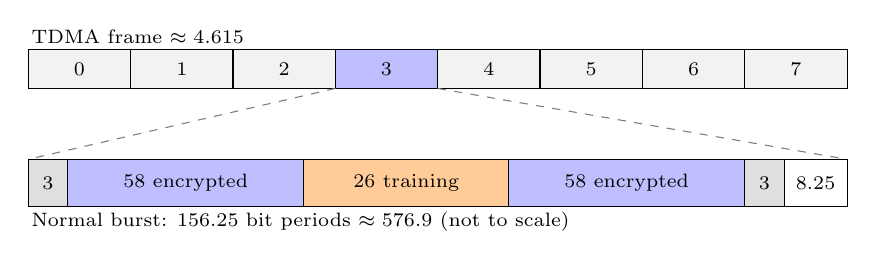
\begin{tikzpicture}[>=latex]
    % TDMA frame
    \foreach \slot in {0,...,7} {
        \draw[fill=gray!10] ({1.3*\slot},1.5) rectangle ({1.3*(\slot+1)},2.0);
        \node[font=\scriptsize] at ({1.3*\slot+0.65},1.75) {\slot};
    }
    \draw[fill=blue!25] (3.9,1.5) rectangle (5.2,2.0);
    \node[font=\scriptsize] at (4.55,1.75) {3};
    \node[anchor=south west, font=\scriptsize, inner sep=1pt] at (0,2.02) {TDMA frame $\approx\qty{4.615}{\milli\second}$};

    % Zoom into one slot
    \draw[dashed, gray] (3.9,1.5) -- (0,0.6);
    \draw[dashed, gray] (5.2,1.5) -- (10.4,0.6);

    % Normal burst, widths are not to scale
    \draw[fill=gray!25] (0,0) rectangle (0.5,0.6);
    \draw[fill=blue!25] (0.5,0) rectangle (3.5,0.6);
    \draw[fill=orange!40] (3.5,0) rectangle (6.1,0.6);
    \draw[fill=blue!25] (6.1,0) rectangle (9.1,0.6);
    \draw[fill=gray!25] (9.1,0) rectangle (9.6,0.6);
    \draw[fill=white] (9.6,0) rectangle (10.4,0.6);

    \node[font=\scriptsize] at (0.25,0.3) {3};
    \node[font=\scriptsize] at (2.0,0.3) {58 encrypted};
    \node[font=\scriptsize] at (4.8,0.3) {26 training};
    \node[font=\scriptsize] at (7.6,0.3) {58 encrypted};
    \node[font=\scriptsize] at (9.35,0.3) {3};
    \node[font=\scriptsize] at (10.0,0.3) {8.25};
    \node[anchor=north west, font=\scriptsize, inner sep=1pt] at (0,-0.03) {Normal burst: \num{156.25} bit periods $\approx\qty{576.9}{\micro\second}$ (not to scale)};
\end{tikzpicture}


  \vspace{0.5em}
  \raggedright
  \begin{itemize}
    \item Training sequence: known bits in the middle of the burst, used to estimate the multipath channel and equalize
    \item Tail bits: define the start and end state of the equalizer
    \item Guard period: absorbs differences in arrival time between users of neighboring slots
    \item Timing advance: terminals far from the base station transmit earlier
  \end{itemize}
\end{frame}

\begin{frame}{Reading the Standard: Normal Burst}
  \begin{columns}[T,onlytextwidth]
    \begin{column}{0.60\textwidth}
      \centering
      \footnotesize
      \begin{tabular}{rrl}
        \toprule
        \textbf{Bit Number} & \textbf{Length} & \textbf{Content} \\
        \midrule
        0--2 & 3 & Tail bits \\
        3--60 & 58 & Encrypted bits ($e_0 \dots e_{57}$) \\
        61--86 & 26 & Training sequence bits \\
        87--144 & 58 & Encrypted bits ($e_{58} \dots e_{115}$) \\
        145--147 & 3 & Tail bits \\
        148-- & 8.25 & Guard period \\
        \bottomrule
      \end{tabular}

      \vspace{0.3em}
      \normalsize
      Normal burst for \gls{acro:gmsk}, adapted from~\cite{ts45002}
    \end{column}
    \begin{column}{0.36\textwidth}
      \begin{block}{How to Read this Table}
        \begin{itemize}
          \item Check: sums to \num{156.25}
          \item Each field refers to another clause or specification
          \item Details such as channel coding are in TS 45.003
        \end{itemize}
      \end{block}
    \end{column}
  \end{columns}
  \vspace{0.5em}
  \begin{itemize}
    \item Specification = exact bit-level contract between independent manufacturers
    \item Rule of thumb: tables and figures first, prose second
    \item Task: find the slot duration and symbol rate in the specifications yourself
  \end{itemize}
\end{frame}

\begin{frame}{GSM Modulation: GMSK}
  \begin{columns}[T,onlytextwidth]
    \begin{column}{0.56\textwidth}
      \Gls{acro:gmsk}~\cite{ts45004}
      \begin{itemize}
        \item Data is filtered by a Gaussian filter before frequency modulation
        \item Bandwidth-time product $BT = 0.3$
        \item Symbol rate $1/T = 1625/6\,\mathrm{ksymb/s}$, one bit per symbol
      \end{itemize}
      \vspace{0.4em}
      Why this Choice?
      \begin{itemize}
        \item Constant envelope: amplifier can run in saturation
        \item High amplifier efficiency extends terminal battery life
        \item Smooth phase gives low out-of-band emissions
      \end{itemize}
    \end{column}
    \begin{column}{0.40\textwidth}
      \begin{block}{Link to Preliminaries}
        \begin{itemize}
          \item Time-frequency uncertainty applies again
          \item Rect pulse: strong sidelobes
          \item Gaussian pulse: compact spectrum, but spreads over several bits
        \end{itemize}
      \end{block}
      \begin{alertblock}{Tradeoff}
        Smaller $BT$ gives a narrower spectrum, but more intersymbol interference.
      \end{alertblock}
    \end{column}
  \end{columns}
\end{frame}

\begin{frame}{GSM Beyond the Air Interface}
  \begin{columns}[T,onlytextwidth]
    \begin{column}{0.54\textwidth}
      New Capabilities
      \begin{itemize}
        \item \Gls{acro:sim}: separates subscriber from device
        \item Roaming across operators and borders
        \item Encryption of the radio link
        \item \Gls{acro:sms}: first mass-market data service
      \end{itemize}
      \vspace{0.4em}
      Rollout
      \begin{itemize}
        \item First GSM call: 1 July 1991 in Finland~\cite{nokia-gsm}
        \item Germany: D-Netz regular operation from 1992~\cite{telekom-gsm}
      \end{itemize}
    \end{column}
    \begin{column}{0.42\textwidth}
      \begin{block}{Other 2G Systems}
        \begin{itemize}
          \item D-AMPS (USA): \gls{acro:tdma} on \gls{acro:amps} channels
          \item PDC (Japan): \gls{acro:tdma}
          \item IS-95 (USA): \gls{acro:cdma}, covered with 3G
        \end{itemize}
      \end{block}
      \begin{alertblock}{Key Insight}
        Roaming results from a common standard, not from digital technology.
      \end{alertblock}
    \end{column}
  \end{columns}
\end{frame}


\subsectionFrame{ETSI and the GSM Standard}

\begin{frame}{From CEPT to ETSI}
  \begin{columns}[T,onlytextwidth]
    \begin{column}{0.58\textwidth}
      \begin{tabular}{ll}
        \toprule
        \textbf{Year} & \textbf{Milestone} \\
        \midrule
        1982 & \acrshort{acro:cept} forms Groupe Spécial Mobile~\cite{3gpp-gsm-history,gsma-history} \\
        1987 & \acrshort{acro:gsm} \acrshort{acro:mou} executed~\cite{etsi-history} \\
        1988 & \Gls{acro:etsi} created (January)~\cite{etsi-history} \\
        1988 & First \gls{acro:gsm} specifications ready~\cite{etsi-history} \\
        1989/90 & \Gls{acro:gsm} work moves to \gls{acro:etsi}~\cite{etsi-history,3gpp-gsm-history} \\
        1991 & First \gls{acro:gsm} call~\cite{nokia-gsm} \\
        1998 & \Gls{acro:3gpp} formed~\cite{3gpp-gsm-history} \\
        \bottomrule
      \end{tabular}
    \end{column}
    \begin{column}{0.38\textwidth}
      \begin{block}{Why a New Body?}
        \begin{itemize}
          \item \Gls{acro:cept} represented administrations
          \item \Gls{acro:etsi} also includes manufacturers and network operators
          \item Pan-European technology needs a pan-European process
        \end{itemize}
      \end{block}
    \end{column}
  \end{columns}
  \vspace{0.5em}
  \alert{Remark:} \Gls{acro:gsm} specifications are maintained in \gls{acro:3gpp} today, which is why TS 45.002 carries a \gls{acro:3gpp} number.
\end{frame}

\begin{frame}{ETSI and Patents: From SEP to FRAND}
  \begin{columns}[T,onlytextwidth]
    \begin{column}{0.58\textwidth}
      The Problem
      \begin{itemize}
        \item 1987, \gls{acro:cept} Patent Panel: a standard may bestow a \enquote{windfall} monopoly on one supplier~\cite{pocknell-etsi}
        \item \Gls{acro:gsm} still contains many \glspl{acro:sep}~\cite{bekkers-gsm}
        \item Motorola refused general licensing declarations and favored cross-licensing~\cite{anagnostopoulos-patents}
      \end{itemize}
      \vspace{0.4em}
      Finding a Policy~\cite{pocknell-etsi}
      \begin{itemize}
        \item Early 1990s: draft \enquote{undertaking}, licensing in advance as a condition of membership
        \item 1993: tentatively approved, never in effect after criticism and a formal complaint
        \item November 1994: simplified \gls{acro:ipr} policy approved
      \end{itemize}
    \end{column}
    \begin{column}{0.38\textwidth}
      \begin{block}{Result: ETSI IPR Policy}
        \begin{itemize}
          \item Members declare essential patents
          \item Holders commit to \gls{acro:frand} licensing
          \item \Gls{acro:frand} terms are not defined further
        \end{itemize}
      \end{block}
      \begin{alertblock}{Scale}
        More than \num{23500} patents declared essential to \gls{acro:gsm}~\cite{ec-sep-brief}
      \end{alertblock}
    \end{column}
  \end{columns}
\end{frame}

\begin{frame}{Summary: Why Cellular and Digital?}
  \centering
  \begin{tabular}{lll}
    \toprule
    \textbf{Shift} & \textbf{Bottleneck} & \textbf{Solution} \\
    \midrule
    Cellular (0G $\rightarrow$ 1G) & Channels usable only once per region & Frequency reuse in cells \\
    Digital (1G $\rightarrow$ 2G) & High required \gls{acro:sir}, no security & Coding, \gls{acro:tdma}, encryption \\
    Common standard & National, incompatible systems & \Gls{acro:gsm} and \gls{acro:etsi} \\
    \bottomrule
  \end{tabular}

  \vspace{1em}
  \begin{alertblock}{Next: 3G}
    \centering
    Voice is solved, data demand is rising. \Gls{acro:tdma} slots are too rigid for this. Is there another way to share the channel?
  \end{alertblock}
\end{frame}
